\chapter{Antecedentes y estado del arte}
\section{Definición}
Se llama realidad aumentada al conjunto de tecnologías que permite a un usuario ver contenido virtual superpuesto al mundo real mediante un dispositivo tecnológico. Las tecnologías de realidad virtual se diferencian en que sumerge al usuario dentro de un entorno completamente sintético, sin tener consciencia del mundo real que lo rodea. La Realidad Aumentada no sustituye la realidad, sino que la complementa y puede mejorar la experiencia en ciertos ámbitos.

\section{Historia}
\begin{wrapfigure}{r}{0.5\textwidth}
    \centering
    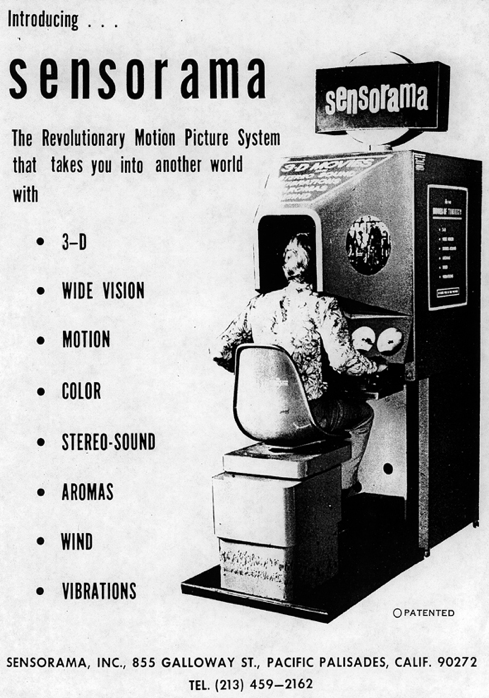
\includegraphics{Images/Sensorama.png}
    \caption{Cartel publicitario de la máquina Sensorama}
    \label{fig:Sensorama}
\end{wrapfigure}

En la década de 1950, surgió por primera vez el término realidad aumentada cuando Morton Heilig, un cinematógrafo, pensó en un prototipo de un cine que estimulara todos los sentidos del ser humano de manera efectiva. Años más tarde, concretamente en el 1962, Heilig construyó dicho prototipo, llamado Sensorama, se trataba de un cine inmersivo y novedoso que incluía funcionalidades como 3D, visión angular (actualmente conocido como IMAX), vídeo en color, sonido en estéreo, además de estimular otros sentidos con aromas, viento, y vibraciones como podemos observar en la figura \ref{fig:Sensorama}.\\
\\
\\
\\
\\
\\

\begin{wrapfigure}{r}{0.5\textwidth}
    \centering
    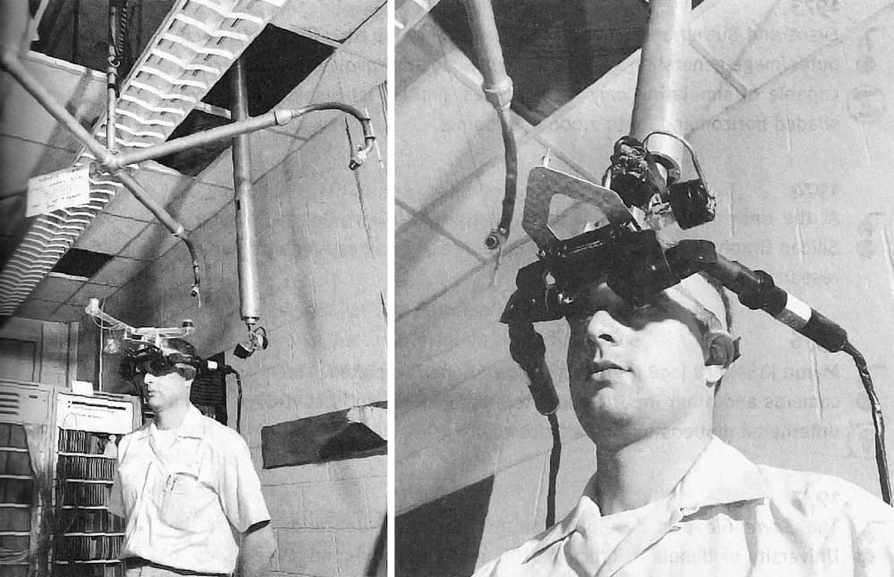
\includegraphics[width=0.48\textwidth]{Images/HumanMountDisplay.png}
    \caption{Ivan Sutherland “Espada de Damocles” 1968.}
    \label{fig:EspadaDamocles}
\end{wrapfigure}

En el 1968, Ivan Sutherland, inventó el HMD (\textit{Human Mounted Display}), siendo así, el primer sistema que permitía ver las aristas de sencillos objetos 3D (\textit{Wireframe}) en tiempo real. Empleaba dos sistemas de \textit{tracking} para calcular el registro de la cámara; uno mecánico y otro basado en ultrasonidos. Debido a su gran peso, se decidió colgar el artefacto en el techo, como se puede ver en la figura \ref{fig:EspadaDamocles}.
\\
\\
\\
\\
\\
\\


Sin embargo, no fue hasta 1992 cuando se acuñó el término de Realidad Aumentada por Tom Caudell y David Mizell, dos ingenieros de Boeing que proponían el uso de esta novedosa tecnología para mejorar la eficiencia y experiencia de las tareas realizadas por operarios humanos asociadas a la fabricación de aviones.
La aparición del primer videojuego en realidad aumentada ocurrió en el año 2000. Bruce Thomas demostró en el ISWC (The International Symposium on Wearable Computers) su videojuego ARQuacke. El sistema empleaba una brújula digital, un receptor de GPS y métodos de visión basados en marcas \cite{ARToolkit}. Los jugadores tenían que llevar una especie de ordenador portátil a la espalda, un casco de visión estereoscópica y un mando de dos botones\cite{ARQuake} como podemos ver en la figura \ref{fig:Dispositivo_ARQuake} . El funcionamiento del HMD, como se puede ver en la figura \ref{fig:HIWARQuake} consistía en un divisor de haz que recibía la imagen virtual desde una pantalla que permitía ver el mundo real y el virtual en los ojos del usuario. La imagen resultante, como se puede observar en la figura \ref{fig:Ex_ARQuake} permitía una inmersión muy lograda para la época.
{\let\thefootnote\relax\footnote{{{Imágenes de las figuras \ref{fig:HIWARQuake} y \ref{fig:Dispositivo_ARQuake} sacadas del libro de ARQuake\cite{ARQuake}  }}}}

{\let\thefootnote\relax\footnote{{Imagen de la figura \ref{fig:Ex_ARQuake} sacada de \url{http://www.tinmith.net/arquake/}}}}


\begin{figure}[ht]
    \centering
    \begin{minipage}{0.32\textwidth}
        \centering
        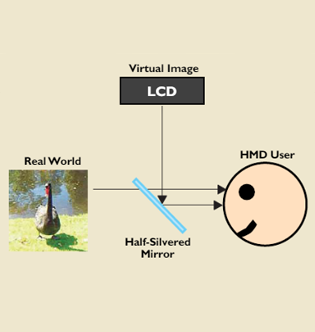
\includegraphics[width=\linewidth]{Images/ARQuake_HIW.png}
        \caption{Funcionamiento del Head Mounted Display}
    \label{fig:HIWARQuake}
    \end{minipage}\hfill
    \begin{minipage}{0.32\textwidth}
        \centering
        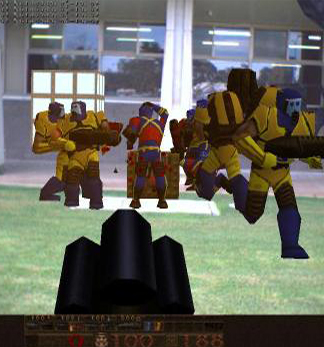
\includegraphics[width=\linewidth]{Images/arquake.jpg}
    \caption{Ejemplo de ARQuake.}
    \label{fig:Ex_ARQuake}
    \end{minipage}
        \begin{minipage}{0.32\textwidth}
        \centering
        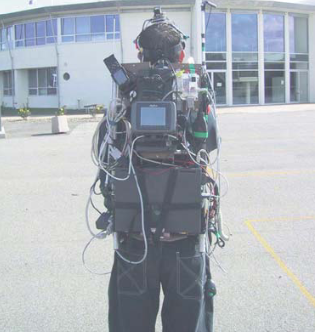
\includegraphics[width=\linewidth]{Images/ARQuake_Dispositivo.png}
    \caption{Dispositivo utilizado para ARQuake}
    \label{fig:Dispositivo_ARQuake}
    \end{minipage}
\end{figure}


En 2007, en el ISMAR(Simposio internacional de realidad aumentada y mixta), Klein y Murray presentan el algoritmo PTAM (Parallel Tracking and Modeling) una variante al SLAM, que separa la localización y el mapeado en hilos diferentes. El SLAM es un algoritmo que sirve para que localizar la posición dentro de un entorno y modelarlo, más tarde lo explicaremos mas a fondo. Separar estos dos procesos en hilos diferentes permitía conseguir unos resultados en tiempo real muy sólidos.\\

\begin{wrapfigure}{r}{0.5\textwidth}
    \centering
    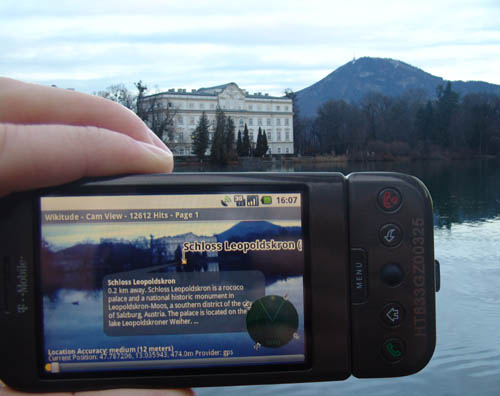
\includegraphics[width=0.48\textwidth]{Images/Wikitude_Example.jpeg}
    \caption{Wikitude App 2008}
    \label{fig:wikitude2008}
\end{wrapfigure}

En 2008 se creó Wikitude, una aplicación que utilizaba el GPS para mostrarte información de la Wikipedia según el lugar en el que estuvieras, pudiendo aprender datos sobre monumentos, esculturas o construcciones que te fueras encontrando. Como se puede ver en la figura \ref{fig:wikitude2008}, el cámara está enfocando un castillo y el móvil le dice cuál es, además le aporta información adicional como la distancia a la que está y el origen del castillo. \\
\\
\\
\\
\\
\\
\\

Un año más tarde, en 2009, desarrolló el videojuego ARhrrrr! del género shooter, el primer videojuego en realidad aumentada para smartphone con contenido 3D de alta calidad. Se generaba un mapa 3D sobre un marcador, y el objetivo era rescatar a los humanos de la ciudad y matar a los zombies (ver figura \ref{fig:arhrrrr})\cite{ARToolkit}.
{\let\thefootnote\relax\footnote{{Imagen de la figura \ref{fig:arhrrrr} sacada de \url{https://github.blairmacintyre.me/site-archive/ael-2015/research/games/arhrrrr/}}}}
\begin{figure}[H]
    \centering
        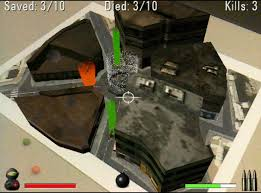
\includegraphics[width=0.5\linewidth]{Images/Arrrr.jpeg}
        \caption{Ejemplo del videojuego ARhrrrr!.}
        \label{fig:arhrrrr}
  \end{figure}
En el mismo año, el estudio español Novorama crea el videojuego de PSP (PlayStation Portable) Invizimals, un éxito mundial, vendiendo más de 8 millones de copias en todo el mundo en el primer trimestre de 2010. Este juego necesita usar la cámara adicional que se conecta a la PSP, y gracias al uso de los marcadores, se puede registrar la posición del jugador.

En 2014, Project Tango nació como uno de los primeros desarrollos de realidad aumentada pensado para ser distribuido mundialmente en los smartphones. En 2015, Tango pasa a formar parte de Google. El objetivo era crear un dispositivo portátil que permitiese mapear espacios 3D. Esta tecnología solo se desarrolló para el dispositivo Phab2 Pro de Lenovo, el cual incluía un mayor número de cámaras, concretamente 3.
Las tres funcionalidades principales para el desarrollo de esta tecnología han sido:
\begin{itemize}
\item Seguimiento del movimiento: Se trata del uso de las características visuales del entorno combinadas con los datos proporcionados por los sensores de movimiento incorporados en el teléfono, el acelerómetro y por el giroscopio, teniendo como objetivo realizar un seguimiento de los movimientos hechos del dispositivo. 
\item Reconocimiento del ambiente: Tango almacena la información del entorno que le rodea, buscando los puntos característicos en cada fotograma que recibe de las cámaras (más adelante explicaremos con más detalle cómo funciona el reconocimiento del ambiente).
\item Percepción de profundidad: Gracias a las cámaras especiales que incorpora el dispositivo, Tango puede calcular tamaños y distancias en el entorno que se encuentra. 
\end{itemize}
Después de 3 años, en 2017, Google decide cerrar el desarrollo de Tango y se centra en su tecnología actual, ARCore, que es el competidor directo de ARKit, la librería de Apple.


\section{Aplicaciones}
En este apartado se recogen las principales aplicaciones por sectores que existen de la realidad aumentada. Estas son la medicina, educación, arte, seguridad, publicidad, turismo, ecommerce y videojuegos.\\
\textbf{FALTA POR RELLENAR ALGÚN EJEMPLO Y SECTOR} 
\subsection{Medicina}
El estrés intenso, incomodidad o la forma de vida sedentaria son factores que tienen un impacto negativo en el bienestar de las personas y su calidad de vida. Se han desarrollado numerosos prototipos para ayudar a la gente con este tipo de problemas. Por otra parte, las técnicas de \textit{gamificación} \footnote{ Técnica de aprendizaje que traslada la mecánica de los juegos al ámbito educativo-profesional con el fin de conseguir mejores resultados.} han sido usadas con éxito en aplicaciones cuyo fin es mejorar la salud de las personas incentivándolas a cambiar sus malos hábitos.\\
Además, ciertos conceptos de juegos de realidad aumentada pueden ser utilizados con propósitos de salud en ancianos. La actividad física es un aspecto clave al hacernos mayores. Algunas consideraciones conceptuales e investigaciones han ayudado a desarrollar entornos de realidad aumentada que sirvan a las personas mayores para hacer ejercicio y mejorar su calidad de vida.\\
Como éste, existen gran variedad de conceptos que implican el uso de la realidad aumentada para favorecer el bienestar y la calidad de vida de las personas\cite{ARGames_Gamification}.
\subsection{Educación}
Los juegos en realidad aumentada, en el sector de la educación, tienen el potencial de abrir el camino a nuevas formas de aprendizaje y adquisición de conocimientos, cambiando así la experiencia del estudio. Aun así, todavía hay algunas dudas sobre cómo los juegos que utilizan la realidad aumentada y sus diseños se basan en géneros ya existentes pueden ser usados para expandir el proceso educativo convencional en el contexto de diversos paradigmas teóricos y modelos utilizados en el aprendizaje clásico. Pese a este desconocimiento, es innegable que los métodos de aprendizaje basados en la gamificación han conseguido una mayor implicación de los estudiantes y un mayor interés por el aprendizaje de nuevas materias\cite{ARGames_Gamification}.\\

\subsection{Arte}
La gamificación es un término que se refiere a la mezcla de juegos con medios interactivos (como la realidad aumentada en este caso) para permitir la transformación de una tarea de aprendizaje u obtención de información digital en una experiencia divertida, accesible y que nos aporte los resultados que estábamos buscando.\\

Uno de los principales inconvenientes que se nos ocurren al pensar en la gamificación aplicada al ámbito de el arte en realidad aumentada es que simplemente no existen demasiados ejemplos viables hasta la fecha, aunque sí encontramos aplicaciones con este potencial para la realidad virtual.
Pese a esto, cabe destacar Membit\cite{MembitYT}, una aplicación fotográfica pública que utiliza la geolocalización del dispositivo. Permite a los usuarios tomar fotos de lugares en una determinada orientación espacial o colocar una imagen en el espacio. Para ver la imagen, el usuario accede a un canal o escanea la zona y se coloca desde la posición en que se tomó la captura. Este es un uso único de la realidad aumentada, que crea ventanas asíncronas de experiencias hacia el pasado del lugar en cuestión\cite{ARGames_Gamification}.

\subsection{Fabricación}
La realidad aumentada es sin duda una herramienta que satisface a los usuarios y cada vez está más presente en nuestra vida cotidiana. La realidad aumentada en la industria es, hoy por hoy, un hecho.\\
Gracias a este tipo de tecnología podemos mejorar el sector industrial y hablar de fábricas inteligentes donde prolifere la conexión entre máquinas y datos, y donde se presente la información al operario en diferentes soportes, que permitan mejorar su trabajo y productividad.\\ 
Una de las principales aplicaciones en este terreno es la formación de los operarios mediante el uso de textos explicativos o imágenes que aparecen en realidad aumentada. Pero tampoco hay que alejarse mucho del ámbito doméstico, ya que nosotros mismos proponemos en nuestro capítulo dedicado al desarrollo de nuestras aplicaciones un manual de montaje de muebles en realidad aumentada, que facilita el entendimiento y mejora la experiencia a la hora de montar los muebles de la casa.\\
Se puede observar en la figura \ref{fig:placenote} algunas de las aplicaciones en la industria, donde se puede señalar dónde hay una avería, o que hay que inspeccionar, muy útiles para compartir información entre trabajadores y no tener malentendidos.
{\let\thefootnote\relax\footnote{{Imagen de la figura \ref{fig:placenote} sacada del canal de Youtube de Placenote SDK \cite{PlacenoteYT}}}}
\begin{figure}[H]
     \centering
     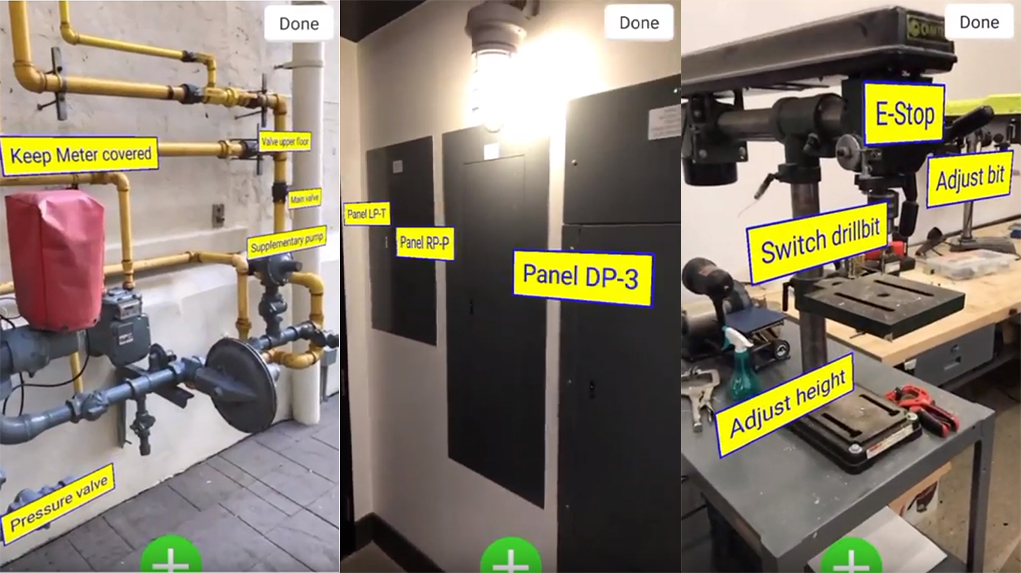
\includegraphics[width=0.7\textwidth]{Images/Placenote.jpg}
     \caption{Ejemplos de uso en la Fabricación.}
     \label{fig:placenote}
 \end{figure}

\subsection{Publicidad}
\subsection{Turismo}
Construir una experiencia de realidad aumentada aplicada al turismo es esencial para el éxito de un destino. El crecimiento en el sector turístico no solo es debido al gran interés cultural y a la gran oferta de ocio que existe, sino también a la velocidad en la que progresa la tecnología y, en particular, la realidad aumentada.\\
Los viajeros pueden interactuar con su entorno gracias a las aplicaciones de turismo de realidad aumentada. De esta forma no sólo están en una localización, sino que se pueden integrar en ella, ya que la realidad aumentada puede crear escenarios que de otra manera sería imposible generar, por ejemplo, recreando edificios o monumentos que en la actualidad ya no existen o están derrumbados.\\
Otra de las aplicaciones más útiles del sector es el traductor de Google, permite traducir un texto con simplemente enfocar a el con la cámara. Como podemos observar en la figura \ref{fig:googletranslate}, su uso es muy cómodo, sobretodo para los idiomas que no utilizan nuestro alfabeto, ya que no hace falta escribir el texto extranjero.

\begin{figure}[H]
     \centering
     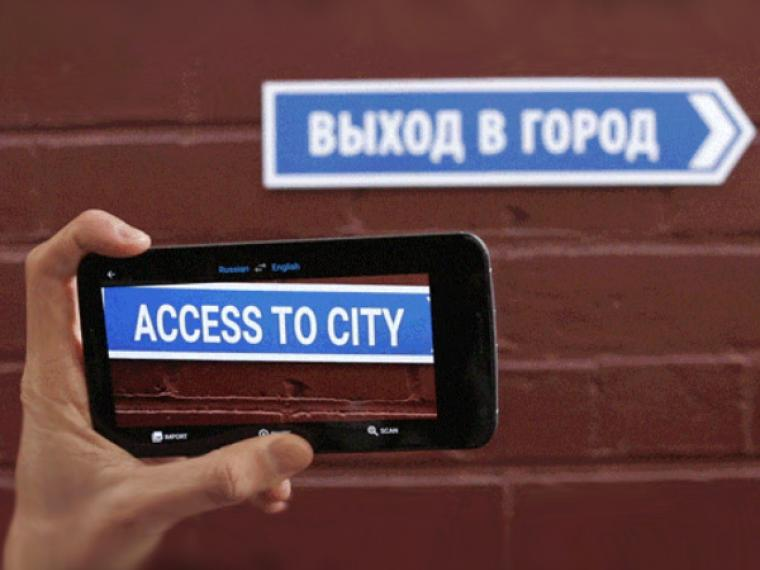
\includegraphics[width=0.7\textwidth]{Images/google-translate.jpg}
     \caption{Google Traductor en RA. Imágenes sacadas de (\url{https://www.muyinteresante.es/tecnologia/articulo/el-nuevo-google-translate-traduce-imagenes-y-voz-211421238921})}
     \label{fig:googletranslate}
 \end{figure}


\subsection{Videojuegos}


\subsection{Comercios electrónicos(ecommerce)}
Los probadores virtuales están marcando tendencia en las nuevas generaciones de aplicaciones y estrategias de venta. Estas aplicaciones hacen uso de la realidad aumentada con tecnologías como el reconocimiento de rostros, reconocimiento de superficies, estimación de luces… Siendo punto de referencia en el mercado los siguientes ejemplos. 
\begin{enumerate}
\item \textbf{Ikea Place}\\
Esta aplicación permite al usuario ver el catálogo de Ikea y una vez seleccionado el elemento verlo en la habitación real con las dimensiones reales del objeto.
\begin{figure}[H]
     \centering
     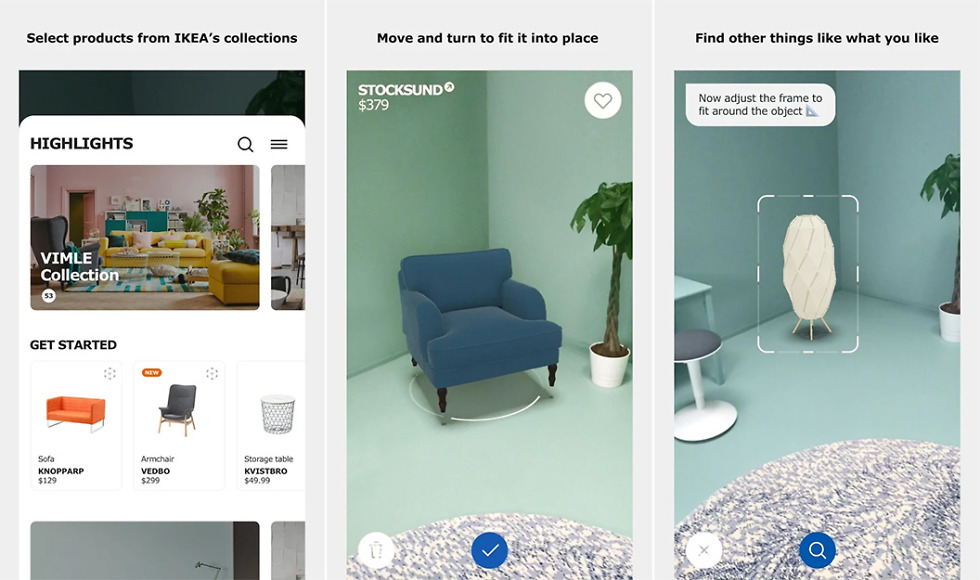
\includegraphics[width=0.6\textwidth]{Images/Ikea_App.jpeg}
     \caption{IKEA Place AR probador virtual}
     \label{fig:Ikea}
 \end{figure}
 \item
 \textbf{YouCam Makeup}\\
Esta aplicación es un excelente y conseguido ejemplo de ecommerce en el mundo de la belleza donde se aplica esta tecnología. La calidad del tracking del pelo es bastante razonable generando una experiencia agradable.
\begin{figure}[H]
    \centering
    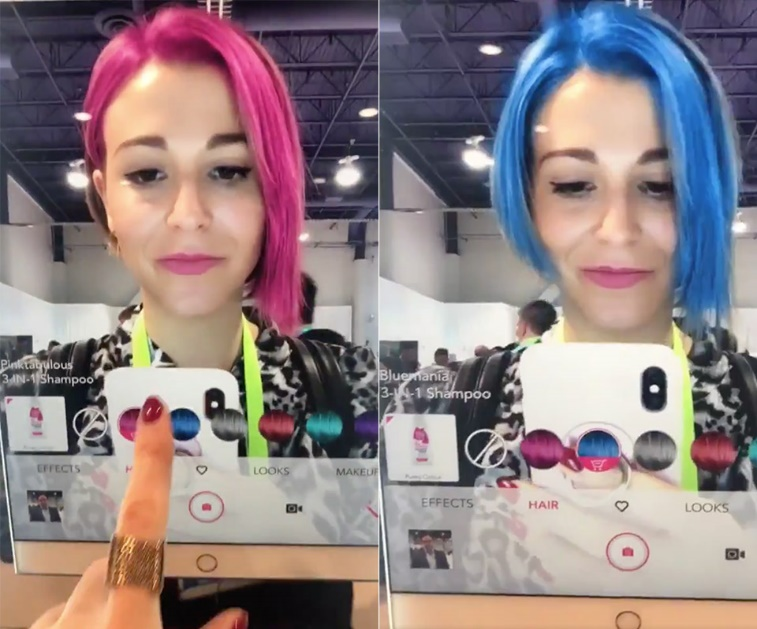
\includegraphics{Images/Loreal_App.jpeg}
    \caption{Imagen representativa de YouCam Makeup}
    \label{fig:YouCam}
\end{figure}
\item \textbf{L’Oreal (Modiface)}\\
Aplicación que permite al usuario maquillarse con los productos de L’Oreal en realidad aumentada, así como escoger el color que más pegue con sus prendas. Mostrando los productos relacionados a esa tonalidad y ofreciendo la posibilidad de comprarlos dentro de la aplicación.
\begin{figure}[H]
    \centering
    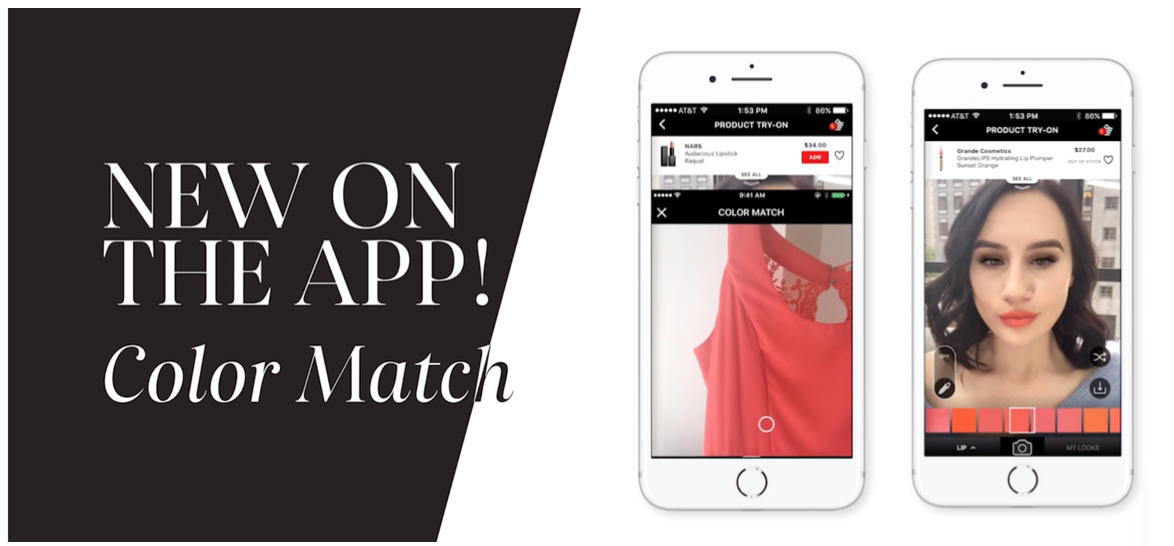
\includegraphics[width=0.7\textwidth]{Images/Loreal_App.png}
    \caption{Pantallas de ejemplo de la aplicación L'Oreal Modiface}
    \label{fig:Loreal}
\end{figure}
\end{enumerate}
\section{Experiencia de usuario en aplicaciones de RA sin marcadores}
\clearpage
\section{
\noindent
